%template1.tex
%The following LaTeX source file represents the simplest kind of slide presentation; no overlays, no included graphics. Substitute your favorite style for ``pascal''. To create the PDF file template1.pdf, (1) be sure to use the prosper class, then (2) execute the command latex template1.tex, and (3) the command dvipdf template1.dvi.

%%%%%%%%%%%%%%%%%%%%%%%%%%%%%%% template1.tex %%%%%%%%%%%%%%%%%%%%%%%%%%%%%%%%%%%
\documentclass[a4paper,blends,pdf,colorBG,slideColor]{prosper}
% definitions for slides for CSC544
% Lutz Hamel, (c) 2007

\hypersetup{pdfpagemode=FullScreen}

\usepackage{times}
\usepackage{latexsym}
\usepackage{alltt}
\usepackage{booktabs}
\usepackage{amsmath}
\usepackage{amsopn}
\usepackage{amsfonts}
\usepackage{amssymb}
%\usepackage[usenames]{color}

\def\sign{\qopname\relax{no}{sign}}
\def\argmax{\qopname\relax{no}{argmax}}
\def\argmin{\qopname\relax{no}{argmin}}

\newcommand{\grad}{\ensuremath{\nabla}} 
\newcommand{\loss}{\ensuremath{{\cal L}}}
\newcommand{\err}{\mbox{err}}
\newcommand{\mse}{\mbox{mse}}
\newcommand{\acc}{\mbox{acc}}
\newcommand{\Integer}{\ensuremath{\mathbb{N}}}
\newcommand{\size}[1]{{|{#1}|}}
\newcommand{\Rnspace}[1]{\ensuremath{\mathbb{R}^{#1}}}
\newcommand{\Real}{\ensuremath{\mathbb{R}}}
\newcommand{\mytt}[1]{{\small\tt{#1}}}
\newcommand{\textemph}[1]{{\em #1}}
\newcommand{\suchthat}{\mid}
\newcommand{\orbar}{\;|\;}
\newcommand{\bs}[1]{\begin{slide}{#1}\ptsize{8}}
\newcommand{\es}{\end{slide}}
\newcommand{\co}{\,\colon\;}
\newcommand{\pair}[2]{\ensuremath{( {#1}, {#2} )}}
\newcommand{\model}[1]{\hat{#1}}
\newcommand{\ul}[1]{{\bf\em #1}}
\newcommand{\ol}{\overline}
\newcommand{\definition}[1]{{\bf Definition: }{\em #1}}
\newcommand{\example}[1]{{\bf Example: }{#1}}
\newcommand{\abs}[1]{|{#1}|}
\newcommand{\mytab}{\makebox[.1in]{}}

\newcommand{\fdef}[1]{
\begin{center}
\fbox{
\begin{minipage}{3.5in}
{\bf Definition:}
{#1}
\end{minipage}
}
\end{center}
}

\newcommand{\fframe}[1]{
\begin{center}
\fbox{
\begin{minipage}{3.5in}
{#1}
\end{minipage}
}
\end{center}
}

\newcommand{\nframe}[1]{
\begin{center}
\begin{minipage}{3.5in}
{#1}
\end{minipage}
\end{center}
}

\newenvironment{Rcode}
	{
		\scriptsize
		\begin{quote}
		\begin{alltt}
	}
	{
		\end{alltt}
		\end{quote}
	}




\begin{document}

\bs{Noisy Data}
Noisy data $\Rightarrow$ small margin.

\begin{center}
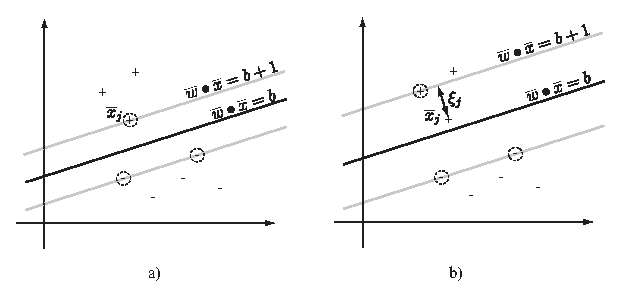
\includegraphics[width=4in]{figures/fig07-04.eps}
\end{center}

Solution: ignore the noisy points.
\es

\bs{Maximum Margin Classifiers}
Recall that our maximum margin classifiers are models of the form
\begin{equation*}
\model{f}(\ol{x}) = \sign\left ( \ol{w} \bullet \ol{x} - b \right ),
\end{equation*}
where the normal vector $\ol{w}$ and the offset term $b$
of the decision surface are computed via the primal optimization problem,
\begin{equation*}
\min \phi(\ol{w},b)  =  \min \frac{1}{2}\ol{w}\bullet\ol{w},
\end{equation*}
subject to the constraints,
\begin{equation*}
y_i(\ol{w}\bullet\ol{x}_i-b) - 1\ge 0,
\end{equation*}
with $i = 1,\ldots, l$ given the training set $(\ol{x}_1,y_1),\ldots,(\ol{x}_l,y_l) \in \Rnspace{n}\times \{+1,-1\}$.
\es

\bs{Softmargin  Classifiers}
\small
If we allow points to lie on the ``wrong'' side of their supporting hyperplanes we need to
keep track  of the amount of error that this introduces $\Rightarrow$ {\em slack variables} 
denoted with $\xi$ (xi) (see Fig b above)

We change our  training algorithm by taking the slack variables into account.  We rewrite our
constraints as
\begin{equation*}
y_i(\ol{w}\bullet\ol{x}_i-b) + {\color{red}\xi_i} - 1 \ge 0,
\end{equation*}
with $\xi_i \ge 0$.

We also modify our objective function,
\begin{equation*}
\min_{\ol{w},\ol{\xi},b} \phi(\ol{w},\ol{\xi},b) 
	=  \min_{\ol{w},\ol{\xi},b}  \left( \frac{1}{2}\ol{w}\bullet\ol{w} + {\color{red}C \sum_{i=1}^{l}\xi_i}\right),
\end{equation*}
Our new objective function looks just like the objective function for maximum margin classifiers
except for the penalty term  $C \sum_{i=1}^{l}\xi_i$.  C is called the {\em cost}. In this way the optimization becomes a trade off between the size of the margin and the size of the error measured by the slack variables,
\begin{equation*}
\boxed{
\begin{aligned}
\text{large $C$} &\sim \text{small margin}\\
\text{small $C$} &\sim \text{large margin}
\end{aligned}
}
\end{equation*}
\es

\bs{Softmargin  Classifiers}
\small
Putting this all together,

\fframe{{\bf Proposition:} [Soft-Margin Optimization]
Given a training set 
\begin{equation*}
D = \{(\ol{x}_1,y_1),(\ol{x}_2,y_2),\ldots,(\ol{x}_l,y_l)\} \subseteq \Rnspace{n} \times \{+1,-1\},
\end{equation*}
we can compute a soft-margin  decision surface $\ol{w}^*\bullet\ol{x} = b^*$ with an optimization,
\begin{equation*}
\min_{\ol{w},\ol{\xi},b} \phi(\ol{w},\ol{\xi},b) 
	=  \min_{\ol{w},\ol{\xi},b}  \left( \frac{1}{2}\ol{w}\bullet\ol{w} + C \sum_{i=1}^{l}\xi_i\right),
\end{equation*}
subject to the constraints,
\begin{align*}
y_i(\ol{w}\bullet\ol{x}_i-b)+ \xi_i - 1 &\ge 0, \\
\xi_i &\ge 0, 
\end{align*}
with $i = 1,\ldots,l$, $\ol{\xi} = (\xi_1,\ldots,\xi_l)$, and $C > 0$.
}
\vspace{.2in}
{\bf Note:} The slack variables have no impact on the form of our model
$
\model{f}(\ol{x}) = \sign(\ol{w}^*\bullet\ol{x} -b^*).
$

\es

\bs{The Dual}
\small
As before we start by constructing the Lagrangian,
\begin{equation*}
\begin{split}
L(\ol{\alpha},\ol{\beta},\ol{w},\ol{\xi},b) & =
	\frac{1}{2}\ol{w}\bullet\ol{w} + C \sum_{i=1}^{l}\xi_i \\
	& \quad - \sum_{i=1}^l\alpha_i (y_i(\ol{w}\bullet\ol{x}_i - b) + \xi_i -1) \\
	& \quad - \sum_{i=1}^l{\color{red}\beta_i}\xi_i
\end{split}
\end{equation*}
We have an additional set of Lagrangian multipliers for the additional constraints.

This gives us the Lagrangian optimization problem,
\begin{equation*}
\max_{\ol{\alpha},\ol{\beta}} \min_{\ol{w},\ol{\xi},b} L(\ol{\alpha},\ol{\beta},\ol{w},\ol{\xi},b),
\end{equation*}
subject to the constraints,
\begin{align*}
\alpha_i &\ge 0,\\
\beta_i &\ge 0,
\end{align*}
for $i = 1,\ldots,l.$

\es

\bs{The Dual}
Since the primal objective function is convex, this Lagrangian has a unique saddle point
and therefore
a solution $\ol{\alpha}^*, \ol{\beta}^*,\ol{w}^*,\ol{\xi}^*, b^*$ has to satisfy the KKT conditions,
\begin{align*}
\frac{\partial L}{\partial \ol{w}}(\ol{\alpha},\ol{\beta}, \ol{w}^*,\ol{\xi},b) &= 0,\\
\frac{\partial L}{\partial \xi_i}(\ol{\alpha},\ol{\beta},\ol{w},\xi^*_i,b) &= 0,\\
\frac{\partial L}{\partial b}(\ol{\alpha},\ol{\beta},\ol{w},\ol{\xi},b^*) &= 0,\\
\alpha^*_i (y_i(\ol{w}^*\bullet\ol{x}_i - b^*) + \xi^*_i -1)&= 0, \\
\beta^*_i\xi^*_i&= 0,\\
y_i(\ol{w}^*\bullet\ol{x}_i - b^*) + \xi^*_i -1&\ge 0, \\
\alpha^*_i &\ge 0,\\
\beta^*_i &\ge 0,\\
\xi^*_i &\ge 0,
\end{align*}
for $i = 1,\ldots,l$.
\es

\bs{The Dual}
\small
Now taking the partial derivatives in terms of the primal variables:
\begin{align*}
\frac{\partial L}{\partial \ol{w}}(\ol{\alpha},\ol{\beta}, \ol{w}^*,\ol{\xi},b) &=
	\ol{w}^* - \sum_{i=1}^l \alpha_i y_i  \ol{x}_i = \ol{0},\\
\frac{\partial L}{\partial b}(\ol{\alpha},\ol{\beta},\ol{w},\ol{\xi},b^*) &=\sum_{i=1}^l \alpha_i y_i = 0,\\
\frac{\partial L}{\partial \xi_i}(\ol{\alpha},\ol{\beta},\ol{w},\xi^*_i,b) &= C - \alpha_i - \beta_i= 0,
\end{align*}
Since both $\alpha_i \ge 0$ and $\beta_i \ge 0$ the last equation implies that
\begin{equation*}
C \ge \alpha_i \ge 0.
\end{equation*}
Putting this all together we can derive the dual,
\begin{equation*}
\phi'(\ol{\alpha}) = 
  \sum_{i=1}^l \alpha_i - 
  \frac{1}{2}\sum_{i=1}^l \sum_{j=1}^l \alpha_i \alpha_j y_i y_j \ol{x}_i \bullet \ol{x}_j.
\end{equation*}
\es

\bs{The Dual}
\small
\fframe{{\bf Proposition} [The Soft-Margin Lagrangian Dual]
Given a soft-margin optimization in primal form (see the beginning of this set of slides)
then the Lagrangian dual optimization for a soft-margin classifier is
\begin{equation*}
\max_{\ol{\alpha}}  \phi'(\ol{\alpha}) = 
  \max_{\ol{\alpha}} \left ( \sum_{i=1}^l \alpha_i - 
  \frac{1}{2}\sum_{i=1}^l \sum_{j=1}^l \alpha_i \alpha_j y_i y_j \ol{x}_i\bullet\ol{x}_j \right )
\end{equation*}
subject to the constraints,
\begin{align*}
\sum_{i=1}^l \alpha_i y_i &= 0, \\
C \ge \alpha_i  &\ge 0,
\end{align*}
with $i = 1,\ldots,l$.  Here, $C$ is the cost constant.
}

\vspace{.2in}
It is remarkable that this dual differs from the hard-margin case only in the range of values the
Lagrangian multipliers can take on: Points in the margin $\alpha_i = C$, points on the supporting
hyperplanes $C > \alpha_i > 0$, and points far away from the decision surface $\alpha_i = 0$.
\es

\bs{Soft-Margin Classifiers}
\scriptsize
\begin{center}
\includegraphics[width=3.8in]{figures/fig07-09.eps}
\end{center}
\begin{alltt}
> svm.model <- svm(Diagnosis~.,
                   data=biomed.df,
                   type="C-classification",
                   cost=1.0,
                   kernel="linear")
\end{alltt}
\es

\bs{Soft-Margin Classifiers}
\scriptsize
\begin{center}
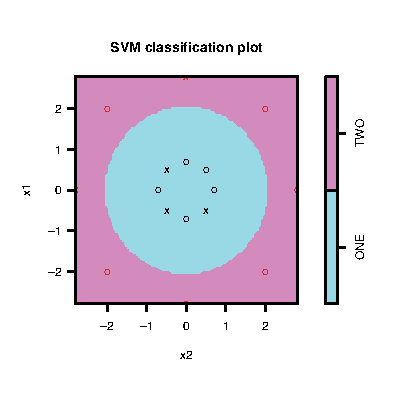
\includegraphics[height=50mm]{figures/fig07-10.eps}
\end{center}
\begin{alltt}
> svm.model <- svm(y~.,
                   data=non.linear.df,
                   type="C-classification",
                   cost=1,
                   kernel="polynomial",
                   degree=2,
                   coef0=0)
\end{alltt}
\es

\bs{Kernel-Perceptron}
\begin{minipage}{2.1in}
\scriptsize
{\bf let} $D = \{(\ol{x}_1,y_1), \dots,(\ol{x}_l,y_l)\} $\\
{\bf let} $0 < \eta <1$\\
$\ol{\alpha} \leftarrow \ol{0}$\\
$b \leftarrow 0$\\
$r \leftarrow \max \{ \abs{\ol{x}} \mid (\ol{x},y)\in D\}$\\
{\bf repeat}\\
\mytab {\bf for} $i = 1$ {\bf to} $l$\\
\mytab\mytab {\bf if} $\sign(\sum_{j=1}^l \alpha_j y_j {\color{red}\ol{x}_j\bullet\ol{x}_i} - b) \neq y_i$ {\bf then}\\
\mytab\mytab\mytab $\alpha_i \leftarrow \alpha_i + 1$\\
\mytab\mytab\mytab $b \leftarrow b - \eta y_i r^2$\\
\mytab\mytab {\bf end if}\\
\mytab {\bf end for}\\
{\bf until done} \\
{\bf return} $(\ol{\alpha}, b)$
\end{minipage}
\begin{minipage}{2in}
\scriptsize
{\bf let} $D = \{(\ol{x}_1,y_1),\dots,(\ol{x}_l,y_l)\} $\\
{\bf let} $\eta > 0$\\
$\ol{\alpha} \leftarrow \ol{0}$\\
$b \leftarrow 0$\\
{\bf repeat}\\
\mytab {\bf for} $i = 1$ {\bf to} $l$ {\bf do}\\
\mytab\mytab {\bf if} $\sign(\sum_{j=1}^l \alpha_j y_j {\color{red}k(\ol{x}_j,\ol{x}_i)} - b) \neq y_i$ {\bf then}\\
\mytab\mytab\mytab $\alpha_i \leftarrow \alpha_i + 1$\\
\mytab\mytab\mytab $b \leftarrow b - \eta y_i$\\
\mytab\mytab {\bf end if}\\
\mytab {\bf end for}\\
{\bf until done} \\
{\bf return} $(\ol{\alpha}, b)$
\end{minipage}

\vspace{.2in}
\small
{\bf Observations:}
\begin{itemize}
\item We extend our linear classifier to a non-linear perceptron.
\item However, sub-optimal decision surface, algorithm stops as soon as a decision surface is found.
\end{itemize}
\es

\end{document}
%%%%%%%%%%%%%%%%%%%%%%%%%%% end of template1.tex %%%%%%%%%%%%%%%%%%%%%%%%%%%%%%%%

